\documentclass[titlepage,a4paper,11pt]{jsarticle}
\usepackage{amsmath,amssymb}
\usepackage{bm}
\usepackage{ascmac}
\usepackage[top=15truemm,bottom=15truemm,left=30truemm,right=30truemm]{geometry}
\usepackage[dvipdfmx]{graphicx}
\usepackage[dvipdfmx]{hyperref}
\pagestyle{empty}

\def\tightlist{\itemsep1pt\parskip0pt\parsep0pt}

\title{発振器とオシロスコープ2}
\date{2017年7月13日}

\begin{document}
\maketitle

\section{実験日・天候}

\begin{itemize}
    \tightlist
  \item
    実験日: 2017年7月6日
  \item
    天候: 晴れ
\end{itemize}

\section{使用機器}

\begin{itemize}
    \tightlist
  \item
    YOKOGAWA デジタルマルチメータ TY710
  \item
    IWATSU デジタル・オシロスコープ DS-5104B
  \item
    KENWOOD 低周波発振器 AG-203D
  \item
    抵抗回路 (製作日: 2017年4月27日)
  \item
    電源回路 (製作日: 2017年5月11日)
\end{itemize}

\section{実験内容}

\subsection{実験1 ダイオードの整流作用}

\subsubsection{実験内容}

まず,発振器を次の設定にした.

\begin{itemize}
    \tightlist
  \item
    波形: 正弦波
  \item
    周波数: 1.0kHz
  \item
    出力: 2.0V(DMMでの表示値)
\end{itemize}

次にこの設定のまま,発振器出力にダイオードと100k\(\Omega\)の負荷抵抗を接続した.

そして,オシロスコープのCH1でダイオードへの入力信号(整流前),CH2でダイオードで整流した後の信号を観測してスケッチをした.

\subsection{実験2 負荷抵抗の影響}

\subsubsection{実験内容}

実験1で,使用している負荷抵抗を100k\(\Omega\)から470\(\Omega\)に交換して,同様に整流前と後の波形をスケッチした.発振器の出力レベルは実験1から変えていない.

\subsection{実験3 矩形波の整流}

\subsubsection{実験内容}

実験2から負荷抵抗を実験1と同じ100k\(\Omega\)に戻し,発振器を次の設定に変えた.

\begin{itemize}
    \tightlist
  \item
    波形: 矩形波
  \item
    周波数: 1.0kHz
  \item
    出力: 2.0V (DMMでの表示値)
\end{itemize}

そして,この時のダイオードへの入力信号(整流前)と整流後の信号をスケッチした.

\section{実験結果}
実験1のスケッチを図1,実験2のスケッチを図2,実験3のスケッチを図3とし,次に表す.

  \begin{figure}[htbp]
    \begin{center}
      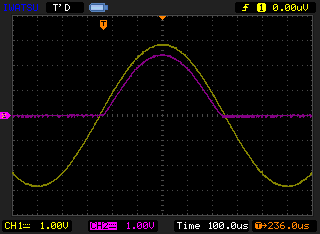
\includegraphics{./img/Copy_0.png}
      \caption{実験1の正弦波の整流波形}
      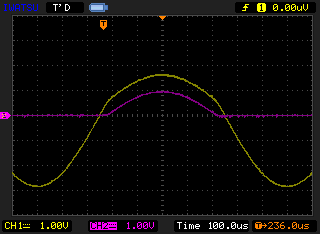
\includegraphics{./img/Copy_1.png}
      \caption{図2: 実験2の整流波形}
      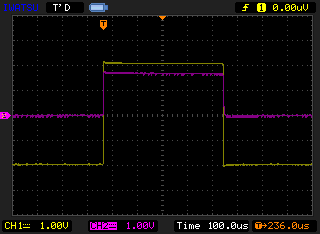
\includegraphics{./img/Copy_2.png}
      \caption{図3: 実験3の矩形波の整流波形}
    \end{center}
  \end{figure}

\newpage

\section{課題}

\subsection{課題1}

図1から,入力電圧(整流前)と整流後の電圧の最大値を読み取った結果,次のようになった.

\begin{itemize}
    \tightlist
  \item
    入力電圧: 2.8V
  \item
    整流後の電圧: 2.4V
\end{itemize}

したがって,その差は \textbf{0.4V}

\subsection{課題2}

発振器の内部抵抗を500\(\Omega\),入力する交流電圧の実効値を2.0Vとすると,100k\(\Omega\)の負荷抵抗をつけた時の回路全体の合成抵抗は100500\(\Omega\)で,回路全体に流れる電流は20\(\mu\)Aとなり,内部抵抗による電圧降下は0.01Vである.

それに対して,500\(\Omega\)の負荷抵抗をつけた時の回路全体の合成抵抗は1000\(\Omega\)で,回路全体に流れる電流は2mAとなり,内部抵抗による電圧降下は1Vとなる.

CH1で観測できる入力電圧は,内部抵抗で電圧降下をした後の値であるので,実験1のように抵抗値大きい負荷抵抗を用いた場合は,回路全体を流れる電流の値が小さくなり,内部抵抗の電圧降下の影響が小さくなったため,波形が歪んでいるように見えなかった.

しかし,実験2では実験1と比較して抵抗値の小さい負荷抵抗をつけたので,回路全体を流れる電流の値が実験1よりも大きくなり,内部抵抗の電圧降下が波形に与える影響が無視できなくなったため,波形の歪みが明らかになったと考えられる.

\subsection{課題3}

実験3では入力信号が矩形波であり,電圧の変化を示した図3のように,回路にかかる電流は,2つの値を一定時間ごとに瞬間的に変化している.そして,ダイオードの順方向電圧降下の値は,順方向電流の値で決まるので,順方向に電流が流れている時,その値は一定で,電圧降下も一定の値を取る.したがって,オシロスコープで観測した入力電圧と整流後の電圧の差は一定となっている.

それに対して,実験1のように入力信号が正弦波のとき,電圧の変化を示した図1のように,回路にかかる電流は,時間とともに周期的に変化している.また,回路全体の合成抵抗値を固定したとき,オームの法則から,電流と電圧は比例関係にあるので,実験1の電流の変化の周期は,電圧の変化の周期と一致する.

したがって,順方向電圧が小さいときは,順方向電流も小さく,ダイオードによる順方向電圧降下も小さい.そして,順方向電圧が大きくなると,順方向電流も大きくなり,ダイオードによる順方向電圧降下も大きくなる.これが入力信号が正弦波のときに,オシロスコープで観測した入力電圧と整流後の電圧の差が一定でない理由である.

\end{document}
